\documentclass[journal]{IEEEtran}
\usepackage[utf8]{inputenc}
\usepackage[T1]{fontenc}
\usepackage{amsmath,amssymb,amsfonts,mathtools}
\usepackage{graphicx}
\usepackage{booktabs,tabularx,array}
\usepackage{cite}
\usepackage{tikz}
\usetikzlibrary{positioning,arrows.meta,calc,fit,backgrounds}
\usepackage{stfloats}
\usepackage{url}
\usepackage[hidelinks]{hyperref}
\usepackage{microtype}

\newtheorem{definition}{Definition}
\newtheorem{proposition}{Proposition}
\newtheorem{corollary}{Corollary}
\newtheorem{remark}{Remark}
\newcommand{\et}{\tilde{\varepsilon}}
\newcommand{\nal}{n_{\alpha}}
\newcommand{\E}{\mathbb{E}}
\newcommand{\passhat}[1]{\mathrm{pass}^{#1}}
\newcommand{\passat}[1]{\mathrm{pass@}#1}
\hyphenation{Web-ridge-AI}

\begin{document}
\bstctlcite{IEEEexample:BSTcontrol}

\title{Lusser's Law for Agents: The Compounding-Reliability Gap in Long-Horizon Agent Harnesses}

\author{Anas~Siddiqui%
\thanks{A. Siddiqui is with WebridgeAI Research, Calgary, AB, Canada.}%
\thanks{Manuscript version 0.2, September 2026. This manuscript is a preprint and has not been peer reviewed. Code and data: \url{https://github.com/big-oh/trust-horizon}.}}

\markboth{Preprint, September 2026}{Siddiqui: Lusser's Law for Agents}

\maketitle

\begin{abstract}
Capability metrics for long-horizon AI agents conceal a large gap between the task length at which an agent succeeds half the time and the length at which it succeeds reliably. The 50\% time horizon of frontier agents has doubled roughly every seven months, yet the 80\% horizon is one quarter to one sixth of it, and the same model weights score 9.5 to 20.8 percentage points apart under different execution harnesses. This paper models a harnessed agent loop as a series reliability system with per-step error, sensors (verifiers) with recall $r$ and false-alarm rate $f$, bounded retries, context degradation, lossy context resets, and checkpoints. Seven results are derived, several by adapting classical reliability results: (i) under constant hazard, the ratio of trust horizon to capability horizon does not depend on model quality; (ii) Gamma-distributed task heterogeneity reproduces the observed ratios and declining hazards without within-task learning; (iii) a sensor multiplies the trust horizon by $G\approx(1-f)/(1-r)$; (iv) retries against a stochastic sensor convert detected failures into silent ones (error laundering); (v) the optimal context-reset interval follows a square-root law analogous to Young's checkpoint interval; (vi) verified checkpoints make expected rerun cost linear rather than exponential in task length; and (vii) a closed-form Trust Horizon Equation combines these effects. Monte Carlo simulation of the same model confirms the closed forms to within 7\%. The model predicts that once verification is strong, the trust horizon grows only as the inverse square root of the sensor miss rate, and handoff fidelity matters as much as sensor recall. No real-agent measurements are reported; six falsifiable hypotheses and a measurement protocol are specified.
\end{abstract}

\begin{IEEEkeywords}
AI agents, harness engineering, large language models, reliability engineering, survival analysis, software verification, checkpointing.
\end{IEEEkeywords}

% =====================================================================================
\section{Introduction}\label{sec:intro}
\IEEEPARstart{I}{n} reliability engineering, the reliability of a system whose components must all function is the product of the component reliabilities, a relation often attributed to Robert Lusser~\cite{oconnor2012}. Ten components that each function with probability 0.95 yield a system that functions with probability 0.60. This relation motivates redundancy in avionics, retries and idempotency in distributed systems, and the ``nines'' vocabulary of site reliability engineering~\cite{beyer2016}.

An AI agent executing a long task is a series system. Every step, whether reading a file, invoking a tool, editing code, or selecting the next action, must succeed, or fail detectably and be repaired, for the task to succeed. An agent with 99\% per-step accuracy therefore completes a 100-step task with probability 0.37 and a 500-step task with probability below 0.01. The model is a component; the loop that executes it is the system.

The engineering of that loop is now called \emph{harness engineering}: the design of the agent loop, context management, tools, memory, feedback and verification, sandboxing, and checkpoints around a model~\cite{lopopolo2026,bockeler2026}. Public leaderboards show that the harness materially affects outcomes. Among Terminal-Bench~2.0 leaderboard submissions compiled by Guo \emph{et al.}, Claude Opus~4.6 scores 58.0\% in one public harness and 76.4\% in another~\cite{guo2026survey}. On SWE-bench Pro, Claude Opus~4.5 scores 45.9\% under a standardized scaffold and 55.4\% under its vendor's harness, a 9.5-point range that is about twice the 4.9-point range spanned by six leading models under the standardized scaffold~\cite{zhang2026disclose}.

Headline evaluations report \emph{capability}: the probability that an agent completes a task in one attempt, or the task length it completes with probability 0.5. Deployment requires \emph{trust}: completion with high probability on every run. The two diverge sharply. In the first release of METR's time-horizon study, the 80\% horizon of the strongest agent measured was about one quarter of its 50\% horizon~\cite{kwa2025v1}; the published version reports 80\% horizons four to six times shorter than 50\% horizons~\cite{kwa2025}. $\tau$-bench reported that GPT-4o's single-trial success of approximately 61\% on retail tasks fell below 25\% when all eight repeated trials were required to succeed~\cite{yao2024}. Practitioner reports describe related failures in long sessions: context silently lost to truncation or compaction, and loops that consume resources without progress~\cite{faafo2026,mindstudio2026,openhands5355}. This paper calls the phenomenon the \emph{run-versus-trust gap} and addresses three research questions:

\begin{itemize}
  \item[RQ1] What functional form does reliability decay take in a harnessed agent loop, and what determines the gap between capability and trust?
  \item[RQ2] Which harness controls (verification, retries, context resets, and checkpoints) extend the trust horizon, by how much, at what cost, and how do they interact?
  \item[RQ3] Which measurements on real agents would confirm or refute the answers?
\end{itemize}

The contributions are as follows.
\begin{enumerate}
  \item A reliability model of the harnessed agent loop in which each harness component corresponds to one parameter: per-step error $\varepsilon_0$, sensor recall $r$ and false-alarm rate $f$, retry budget $m$, context-degradation rate $\gamma$, handoff loss $\rho$, and reset interval $L$ (Section~\ref{sec:model}).
  \item An invariance result for the trust-to-capability ratio, and a frailty account that reproduces the observed ratio and declining population hazards without within-task improvement (Sections~\ref{sec:lusser}--\ref{sec:frailty}).
  \item Closed forms for the verification gain, the error-laundering effect of retries, the square-root law for context resets, and the cost reduction from checkpoints (Sections~\ref{sec:sensors}--\ref{sec:checkpoints}).
  \item The Trust Horizon Equation and a corollary predicting a transition from verification-limited to memory-limited reliability (Section~\ref{sec:the}).
  \item A Monte Carlo study that checks each closed form and characterizes interactions between controls (Section~\ref{sec:sim}).
  \item Six falsifiable hypotheses and a measurement protocol (Section~\ref{sec:program}).
\end{enumerate}

\emph{Scope:} All results are analytical or simulated; no measurements of real agents are reported. The parameter values used in the simulations are illustrative and were not estimated from any deployed agent. The contribution is the functional form of the predictions (which levers act multiplicatively, which have square-root returns, and which interact), each of which can be tested with the protocol of Section~\ref{sec:program}.

% =====================================================================================
\section{Background and Related Work}\label{sec:background}

\subsection{Harness Engineering}
OpenAI's report on building an internal beta product of roughly one million lines with no manually written code describes the engineers' primary job as designing environments, specifying intent, and building feedback loops rather than writing code, and calls this work harness engineering~\cite{lopopolo2026}. B\"ockeler divides a harness into \emph{guides}, feedforward controls such as instructions, architecture maps, and tool schemas that raise the probability of a correct action, and \emph{sensors}, feedback controls such as tests, linters, and review agents that observe outputs and enable self-correction~\cite{bockeler2026}. B\"ockeler and Ford further argue that computational (deterministic) sensors give more assurance than inferential (model-based) ones wherever a check can be made objective~\cite{bockeler2026b}. Anthropic's engineering guidance addresses composable agent patterns~\cite{anthropic2024}, context engineering~\cite{anthropic2025ctx}, tool design~\cite{anthropic2025tools}, and a two-stage harness for long-running tasks in which an initializer prepares the environment and a coding agent makes incremental, tested, committed progress recorded in a progress file~\cite{anthropic2025long}. Models are increasingly post-trained with specific harnesses in the loop, which couples the two, so a model may behave differently under an unfamiliar harness~\cite{oreilly2026}. Guo \emph{et al.}~\cite{guo2026survey} survey agent systems through a model--harness lens and decompose the harness into six runtime responsibilities. Zhang \emph{et al.}~\cite{zhang2026disclose} treat the harness as the controller of a closed-loop system in which the language model acts as a stochastic policy, define controller-level quantities (stability, context drift, and control lag), argue that harness configuration is the binding constraint on performance for frontier-comparable models, and propose disclosure standards. The present work is complementary: it uses a reliability and survival-analysis formulation that yields closed-form horizons and quantitative predictions for individual harness controls.

\subsection{Measuring Agent Reliability}
The pass@$k$ metric is the probability that at least one of $k$ attempts succeeds~\cite{chen2021}. The pass$^k$ metric introduced with $\tau$-bench is the probability that all $k$ attempts succeed~\cite{yao2024}. METR's time horizon is the human-time length of tasks completed with a given probability, estimated with a logistic model in log task length~\cite{kwa2025}. Ord showed that these data are approximately consistent with a constant hazard per unit of human-equivalent work~\cite{ord2025}. Hamilton then fitted Weibull survival models to the same data and found shape parameters below 1 for every agent, between 0.6 and 0.9 for state-of-the-art models and approximately 0.37 for humans, indicating hazard that declines over the course of a task~\cite{hamilton2026}. Ord summarizes the agent values as clustered around 0.6 and notes that Weibull and log-logistic fits differ by a factor of about 20 in their implied 99\% horizons~\cite{ord2026}. The Holistic Agent Leaderboard reports accuracy--cost trade-offs across models and scaffolds~\cite{hal2026}.

\subsection{Verification and Self-Correction}
Intrinsic self-correction without external feedback often fails to improve, and can degrade, reasoning performance~\cite{huang2024}. External verification is more effective: in SWE-Gym, a trained verifier used to select among sampled trajectories improved SWE-bench Verified resolution by 11.4 percentage points~\cite{pan2025}, and weak verifiers are frequently the limiting factor in self-correction~\cite{zhang2024}. Wei's verifier's rule holds that the ease of training AI for a task is proportional to the task's verifiability~\cite{wei2025}; Karpathy makes a related argument about which work is automated first~\cite{karpathy2025}.

\subsection{Context Degradation}
Model accuracy decreases as input length grows, even for simple retrieval~\cite{liu2024,hong2025}. A study of 18 models found performance becoming increasingly unreliable with input length at fixed task difficulty~\cite{hong2025}. Harnesses mitigate this with compaction (summarizing history) and resets (restarting from a structured handoff). One practitioner analysis of long coding sessions found that tool results made up 68\% of the context and that compaction discarded them irrecoverably~\cite{faafo2026}. Anthropic reports that compaction alone is insufficient for multi-session tasks and structures such work as fresh sessions that resume from a progress file and version-control history~\cite{anthropic2025long}.

\subsection{Reliability Engineering Foundations}
Three classical results are used. The reliability of a series system is the product of its component reliabilities~\cite{oconnor2012}. In survival analysis, a population whose members differ in individual hazard (frailty) exhibits declining population hazard even when each individual hazard is constant, because frail members fail first~\cite{vaupel1979}. In high-performance computing, the optimal checkpoint interval balances checkpoint cost against failure rate and follows a square-root law~\cite{young1974,daly2006}.

\begin{table*}[!t]
\centering
\caption{Evidence for the Run-Versus-Trust Gap. Figures as Reported in the Cited Sources}
\label{tab:evidence}
\small
\begin{tabularx}{\textwidth}{@{}p{3.3cm}Xp{2.2cm}@{}}
\toprule
Phenomenon & Evidence & Source\\
\midrule
Harness-induced variance & Identical weights: 58.0\% vs.\ 76.4\% (Claude Opus~4.6) and 59.4\% vs.\ 80.2\% (Gemini~3.1 Pro) among Terminal-Bench~2.0 leaderboard entries; 45.9\% vs.\ 55.4\% (Claude Opus~4.5) on SWE-bench Pro & \cite{guo2026survey,zhang2026disclose}\\
Capability vs.\ trust & Claude~3.7 Sonnet: 59~min at 50\% vs.\ 15~min at 80\% reliability (first release); 80\% horizons 4--6$\times$ shorter than 50\% horizons (published version) & \cite{kwa2025v1,kwa2025}\\
Declining hazard & Weibull shape below 1 for every agent measured (0.6--0.9 for state-of-the-art models); humans $\approx0.37$ & \cite{hamilton2026,ord2026}\\
Inconsistency & GPT-4o, retail: pass$^1$ 0.604 and pass$^4$ 0.383 (repository leaderboard); pass$^8<0.25$ (original paper, separate run) & \cite{taubenchlb,yao2024}\\
Context degradation & Accuracy decreases with input length across 18 models at fixed difficulty & \cite{hong2025,liu2024}\\
Lossy compaction & Tool results made up 68\% of context in long coding sessions; compaction discarded them irrecoverably & \cite{faafo2026}\\
Stuck loops & Loop detectors terminate legitimate long runs; a malformed tool result can permanently stall a session & \cite{openhands5355,openhands5225}\\
Verifier leverage & External verifier: $+11.4$ points; intrinsic self-correction can degrade accuracy & \cite{pan2025,huang2024}\\
\bottomrule
\end{tabularx}
\end{table*}

% =====================================================================================
\section{Problem Statement}\label{sec:problem}
\emph{Agent reliability decays rapidly with task length, so the horizon at which an agent can be trusted lags far behind the horizon at which it is capable. It is not known which harness controls most efficiently slow this decay, how they interact, or what each is worth per unit cost.}

Fig.~\ref{fig:swings} summarizes harness-induced variance: for fixed weights, the choice of harness changes task success by 9.5 to 20.8 percentage points. These comparisons are observational, since public harnesses differ along many dimensions at once; they establish that the harness matters but not which component is responsible. The capability--trust gap is quantified by METR's data and appears in repeated-trial form in $\tau$-bench (Section~\ref{sec:frailty}). The failure modes most often reported by practitioners, namely context loss, silent drift, stuck loops, and brittle recovery, are failures of the loop rather than of any single model invocation (Table~\ref{tab:evidence}).

Prior work measures the decay curve~\cite{kwa2025}, measures inconsistency~\cite{yao2024}, documents harness variance~\cite{hal2026,zhang2026disclose}, or defines controller-level quantities without relating them to horizons~\cite{zhang2026disclose}. To the author's knowledge, no prior work derives how individual harness controls change the reliability-decay curve or predicts the effect of a specific harness change on the trust horizon. Practitioner guidance to add sensors, compact less, or commit progress remains qualitative.

\begin{figure*}[!t]
\centering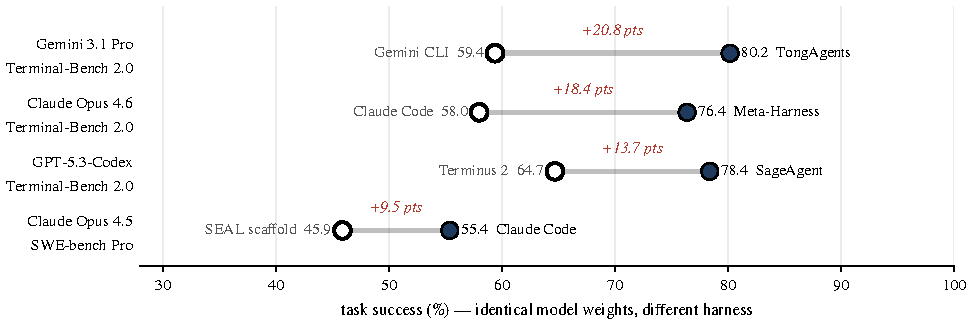
\includegraphics[width=\textwidth]{figs_ieee/fig_swings.pdf}
\caption{Task success for identical model weights under different harnesses. Hollow markers: lower-scoring public harness; filled markers: higher-scoring harness. Terminal-Bench~2.0 leaderboard entries as compiled in~\cite{guo2026survey}; SWE-bench Pro data from~\cite{zhang2026disclose}, who draw on a public leaderboard. Differences are observational, not controlled ablations.}
\label{fig:swings}
\end{figure*}

% =====================================================================================
\section{Reliability Model of the Harnessed Agent Loop}\label{sec:model}

\subsection{Model Definition}\label{sec:setup}
A task comprises $n$ steps, where a step is a unit of progress on which the remainder of the task depends. In the protocol of Section~\ref{sec:program}, steps are operationalized as verifiable intermediate states. Fig.~\ref{fig:anatomy} maps each harness component to its model parameter. The terms \emph{sensor} and \emph{verifier} are used interchangeably for any check applied to an attempt's output.

\begin{figure*}[!t]
\centering
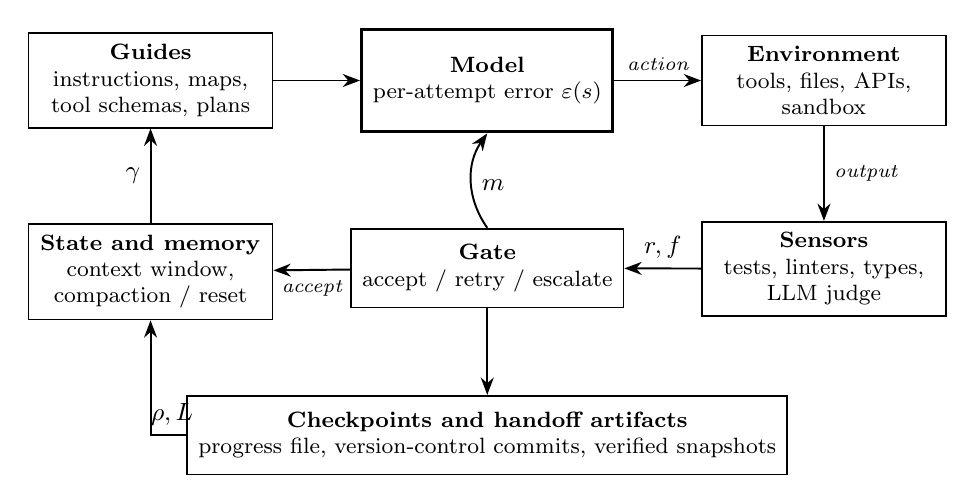
\begin{tikzpicture}[
  font=\footnotesize,
  box/.style={draw=black,line width=0.6pt,align=center,minimum height=10mm,inner sep=4pt,fill=white},
  par/.style={font=\small},
  lab/.style={font=\scriptsize\itshape},
  ar/.style={-{Stealth[length=2.2mm]},line width=0.7pt},
  node distance=8mm and 11mm]
  \node[box,line width=1.2pt,minimum width=28mm,minimum height=13mm] (model) {\textbf{Model}\\ per-attempt error $\varepsilon(s)$};
  \node[box,left=of model,minimum width=31mm] (guides) {\textbf{Guides}\\ instructions, maps,\\ tool schemas, plans};
  \node[box,right=of model,minimum width=31mm] (env) {\textbf{Environment}\\ tools, files, APIs,\\ sandbox};
  \node[box,below=12mm of env,minimum width=31mm] (sensor) {\textbf{Sensors}\\ tests, linters, types,\\ LLM judge};
  \node[box,below=12mm of model,minimum width=28mm] (gate) {\textbf{Gate}\\ accept / retry / escalate};
  \node[box,below=12mm of guides,minimum width=31mm] (state) {\textbf{State and memory}\\ context window,\\ compaction / reset};
  \node[box,below=11mm of gate,minimum width=62mm] (ckpt) {\textbf{Checkpoints and handoff artifacts}\\ progress file, version-control commits, verified snapshots};
  \draw[ar] (guides) -- (model);
  \draw[ar] (model) -- node[above,lab]{action} (env);
  \draw[ar] (env) -- node[right,lab]{output} (sensor);
  \draw[ar] (sensor) -- node[above,par]{$r,f$} (gate);
  \draw[ar] (gate) -- node[below,lab]{accept} (state);
  \draw[ar] (state) -- node[left,par]{$\gamma$} (guides);
  \draw[ar] (gate.north) to[bend left=35] node[right,par,pos=0.45]{$m$} (model.south);
  \draw[ar] (gate) -- (ckpt);
  \draw[ar] (ckpt.west) -| node[above,par,pos=0.2]{$\rho,L$} (state.south);
\end{tikzpicture}
\caption{Harnessed agent loop and the model parameter associated with each component. Guides and context determine the per-attempt error $\varepsilon$; sensors have recall $r$ and false-alarm rate $f$; the gate permits up to $m$ attempts per step; context degrades at rate $\gamma$; resets every $L$ steps lose task-critical state with probability $\rho$.}
\label{fig:anatomy}
\end{figure*}

\begin{definition}[Harnessed loop]\label{def:model}
At each step the agent makes up to $m$ attempts. An attempt made $s$ steps after the most recent context reset is incorrect with probability $\varepsilon(s)=\varepsilon_0(1+\gamma s)$. A sensor flags an incorrect attempt with probability $r$ (recall) and a correct attempt with probability $f$ (false-alarm rate). An unflagged attempt is accepted. A flagged attempt is retried if attempts remain and is otherwise escalated, which constitutes a detected failure. An accepted incorrect attempt is a silent error. The context may be reset every $L$ steps; each reset loses task-critical state with probability $\rho$ (handoff loss), which also constitutes a silent error. A task succeeds if all $n$ steps are accepted correctly.
\end{definition}

With one attempt, no sensor, and no degradation, the model reduces to $n$ Bernoulli trials with success probability $p=1-\varepsilon_0$.

\emph{Assumptions:} The definition makes six assumptions explicit.
(A1)~Series structure: the task fails at its first silent error; this is conservative for agents that later notice and repair mistakes.
(A2)~Given the step and the context age, attempts and sensor verdicts are independent; Sections~\ref{sec:frailty} and~\ref{sec:laundering} relax this across tasks and across retries.
(A3)~Retries do not age the context: $s$ counts completed steps, not attempts.
(A4)~An escalation ends the task and counts as a failure for the trust horizon, although in deployment it is safer than a silent failure because it is visible.
(A5)~Handoff loss is not observable by the step-level sensor.
(A6)~Degradation is linear in context age.

\begin{definition}[Trust horizon]\label{def:horizon}
For a reliability target $\alpha\in(0,1)$, the trust horizon $\nal$ is the largest task length for which the success probability $R(n)$ is at least $\alpha$. The capability horizon is $n_{0.5}$; unless otherwise specified, the trust horizon refers to $n_{0.8}$. The hazard is the per-step failure rate $h=-\tfrac{d}{dn}\ln R(n)$.
\end{definition}

\subsection{Series Reliability and Invariance of the Gap}\label{sec:lusser}

\begin{proposition}[Invariance]\label{prop:invariance}
Under constant per-step error $\varepsilon$, $R(n)=(1-\varepsilon)^n$, and for reliability levels $\alpha$ and $\beta$
\begin{equation}\label{eq:horizon}
\nal=\frac{\ln(1/\alpha)}{-\ln(1-\varepsilon)}\approx\frac{\ln(1/\alpha)}{\varepsilon},\qquad
\frac{n_{\alpha}}{n_{\beta}}=\frac{\ln\alpha}{\ln\beta}.
\end{equation}
In particular, $n_{0.8}/n_{0.5}=\ln 0.8/\ln 0.5\approx0.322$ and $n_{0.99}/n_{0.5}\approx0.0145$, independent of $\varepsilon$.
\end{proposition}

Horizons therefore scale as $1/\varepsilon$: halving per-step error doubles every horizon, but under a constant hazard no improvement in the model or the sensor alters the ratio of trust horizon to capability horizon, as Ord observed for METR's data~\cite{ord2025}. The ratio changes only when failure is not memoryless: heterogeneity across tasks lowers it (Section~\ref{sec:frailty}), and degradation within a task raises it (Section~\ref{sec:rot}). Fig.~\ref{fig:lusser} and Table~\ref{tab:nines} quantify the per-step reliability required.

\begin{figure*}[!t]
\centering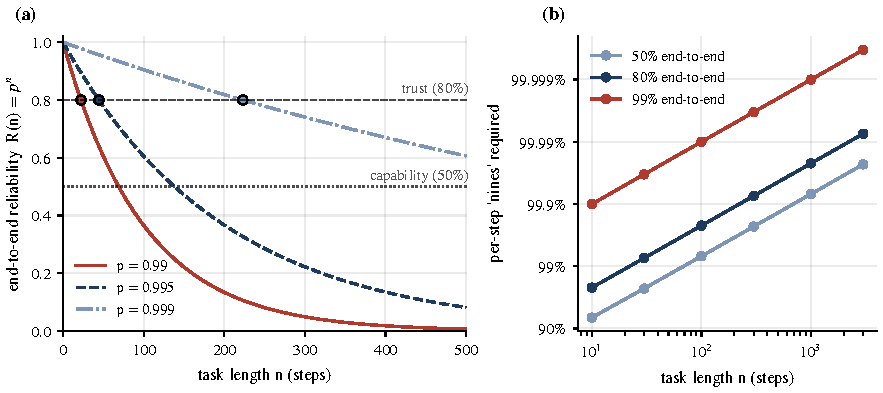
\includegraphics[width=\textwidth]{figs_ieee/fig_lusser.pdf}
\caption{Series reliability of agent loops. (a) End-to-end reliability $R(n)=p^n$ for three per-step reliabilities; circles mark the 80\% trust horizon ($n_{0.8}=22$, $44$, and $223$). (b) Per-step reliability required to reach a given end-to-end reliability; a 1000-step task at 99\% end-to-end reliability requires 99.999\% per step.}
\label{fig:lusser}
\end{figure*}

\begin{table}[!t]
\centering
\caption{Per-Step Reliability $p=\alpha^{1/n}$ Required for End-to-End Reliability $\alpha$ Over $n$ Steps}
\label{tab:nines}
\begin{tabular}{@{}lccc@{}}
\toprule
 & $n=10$ & $n=100$ & $n=1000$\\
\midrule
$\alpha=0.50$ & 93.30\% & 99.31\% & 99.931\%\\
$\alpha=0.80$ & 97.79\% & 99.78\% & 99.978\%\\
$\alpha=0.99$ & 99.90\% & 99.990\% & 99.9990\%\\
\bottomrule
\end{tabular}
\end{table}

\subsection{Task Heterogeneity and Declining Hazard}\label{sec:frailty}
METR's first release gives a ratio of 0.25 for Claude~3.7 Sonnet (15 versus 59~min) rather than 0.32~\cite{kwa2025v1}, the published version reports ratios of about 1/4 to 1/6~\cite{kwa2025}, and Weibull fits indicate hazard that declines over a task~\cite{hamilton2026,ord2026}. One interpretation is that agents improve during a task. Proposition~\ref{prop:frailty} gives an alternative based on heterogeneity across tasks.

\begin{proposition}[Frailty]\label{prop:frailty}
Suppose each task has a constant hazard $\lambda$ per unit length and $\lambda\sim\mathrm{Gamma}(\nu,\omega)$ across tasks, with shape $\nu$ and rate $\omega$. Then the population survival function and hazard are
\begin{equation}\label{eq:frailty}
S(t)=\Bigl(1+\frac{t}{\omega}\Bigr)^{-\nu},\qquad h(t)=\frac{\nu}{\omega+t},
\end{equation}
so the population hazard declines although no individual hazard does. Horizons satisfy $T_\alpha=\omega(\alpha^{-1/\nu}-1)$ and
\begin{equation}\label{eq:frailtyratio}
\frac{T_{0.8}}{T_{0.5}}=\frac{1.25^{1/\nu}-1}{2^{1/\nu}-1},
\end{equation}
which equals $0.25$ exactly at $\nu=1$, where $S$ is log-logistic with unit shape, equals $1/5$ and $1/6$ at $\nu\approx0.56$ and $0.42$, and tends to $0.322$ as $\nu\to\infty$.
\end{proposition}

This effect is well established in demography~\cite{vaupel1979}. The Weibull analyses above interpret a shape below 1 in terms of within-task dynamics such as error correction~\cite{hamilton2026,ord2026}; to the author's knowledge, the selection explanation has not been examined for agent evaluations. The distinction matters because the two interpretations imply different harness designs. If agents improve within a task, runs that survive their early steps face lower hazard, and persistence is rewarded. If the decline reflects selection, whereby difficult tasks fail early, each difficult task retains its full hazard, and retries are less effective than they appear. Population survival curves cannot distinguish the two; repeated trials of the same task can.

\begin{proposition}[pass$^k$ under heterogeneity]\label{prop:passk}
Let the per-trial success probability of a task be $\theta\sim\mathrm{Beta}(a,b)$ across tasks, with trials conditionally independent given $\theta$. Then
\begin{align}
\passhat{k}&=\E[\theta^k]=\prod_{j=0}^{k-1}\frac{a+j}{a+b+j},\label{eq:passk}\\
\passat{k}&=1-\prod_{j=0}^{k-1}\frac{b+j}{a+b+j},\label{eq:passat}
\end{align}
and the intra-task correlation $\kappa=1/(a+b+1)$ is the fraction of outcome variance attributable to task identity. Homogeneous tasks correspond to $\kappa\to0$, for which $\passhat{k}\to p^k$.
\end{proposition}

Fitting (\ref{eq:passk}) to the (pass$^1$, pass$^4$) pairs on the $\tau$-bench repository leaderboard~\cite{taubenchlb} yields $\kappa\approx0.45$--$0.51$ (Table~\ref{tab:beta}): about half of the outcome variance is explained by task identity rather than run-to-run variation. The fit predicts pass$^8=0.30$ for GPT-4o on retail tasks, compared with 0.018 under independence. The original paper reports pass$^8$ below 0.25~\cite{yao2024}, an order of magnitude closer to the heterogeneous prediction but somewhat lower; because that value comes from a separate run (pass$^1=0.612$), the comparison is indicative only. Fig.~\ref{fig:passk}(b) illustrates the consequence for retries. With a perfect selector and independent failures, eight attempts would raise GPT-4o's retail success to 99.94\%; under the fitted heterogeneity, (\ref{eq:passat}) gives 87\%. This difference is called the \emph{retry gap}. The heterogeneity that produces an apparently declining hazard also makes retries less effective than independent-trial calculations indicate.

\begin{table}[!t]
\centering
\caption{Beta-Heterogeneity Fits to $\tau$-Bench Leaderboard Values~\cite{taubenchlb}}
\label{tab:beta}
\setlength{\tabcolsep}{3.2pt}
\begin{tabular}{@{}lcccccc@{}}
\toprule
Agent, domain & p$^1$ & p$^4$ & i.i.d.\ p$^4$ & $\kappa$ & p$^8$ & p@8\\
\midrule
GPT-4o, retail & 0.604 & 0.383 & 0.133 & 0.51 & 0.30 & 0.87\\
Claude 3.5 S., retail & 0.692 & 0.462 & 0.229 & 0.45 & 0.36 & 0.94\\
Claude 3.5 S., airline & 0.460 & 0.225 & 0.045 & 0.47 & 0.15 & 0.79\\
\bottomrule
\multicolumn{7}{@{}p{0.95\columnwidth}@{}}{\footnotesize p$^k$: pass$^k$; p@8: pass@8. p$^1$ and p$^4$ are leaderboard values for tool-calling agents (Claude 3.5 Sonnet: 2024-10-22 release) on the original task set, which was subsequently revised; p$^8$ and p@8 are model predictions.}
\end{tabular}
\end{table}

\begin{figure*}[!t]
\centering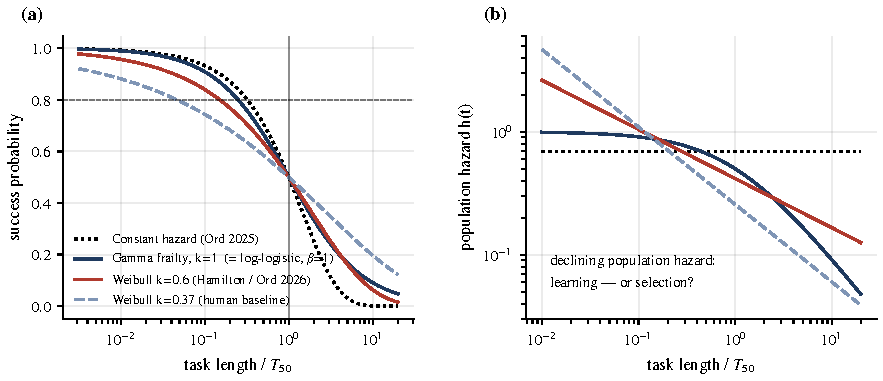
\includegraphics[width=\textwidth]{figs_ieee/fig_frailty.pdf}
\caption{Reliability-decay shapes normalized to a common 50\% horizon. (a) Survival functions; the dashed line marks 80\%. (b) Population hazard. Constant hazard is flat; Gamma frailty and Weibull hazards with shape $\nu<1$ both decline. The curves agree near $T_{50}$ and differ by more than an order of magnitude in their implied 99\% horizons.}
\label{fig:frailty}
\end{figure*}

\begin{figure*}[!t]
\centering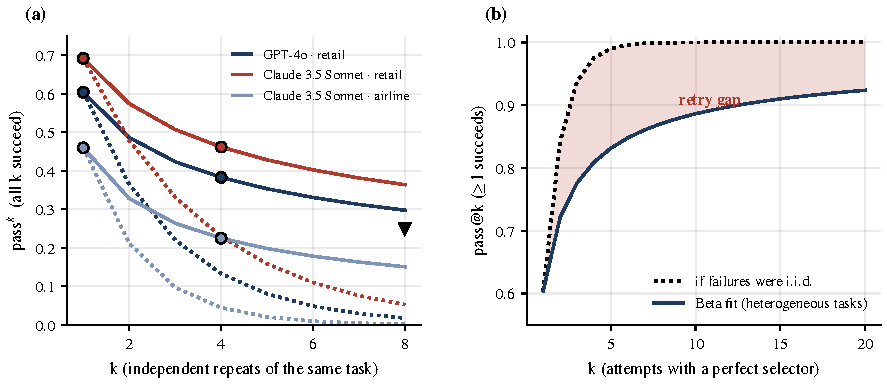
\includegraphics[width=\textwidth]{figs_ieee/fig_passk.pdf}
\caption{Consistency under task heterogeneity. (a) pass$^k$: leaderboard values (circles), Beta fits (solid), and independent-trial prediction $p^k$ (dotted); the triangle marks the bound pass$^8<0.25$ reported for GPT-4o on retail tasks in a separate run~\cite{yao2024}. (b) pass@$k$ for GPT-4o on retail tasks; the shaded region is the retry gap.}
\label{fig:passk}
\end{figure*}

\subsection{Verification With Bounded Retries}\label{sec:sensors}
Fig.~\ref{fig:markov} represents one step, with constant error $\varepsilon$, as a Markov chain. Each attempt terminates in one of three states with probabilities
\begin{align}
a&=(1-\varepsilon)(1-f)\quad\text{(accept, correct)},\nonumber\\
b&=\varepsilon(1-r)\quad\text{(accept, incorrect)},\label{eq:abc}\\
c&=(1-\varepsilon)f+\varepsilon r\quad\text{(reject)}.\nonumber
\end{align}

\begin{figure*}[!t]
\centering
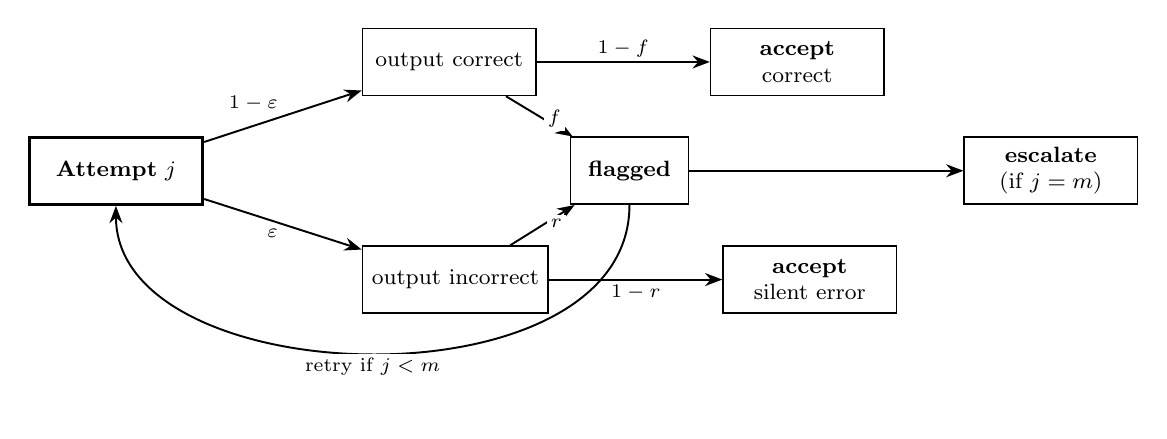
\begin{tikzpicture}[font=\footnotesize,
  st/.style={draw=black,line width=0.6pt,align=center,minimum height=8.5mm,minimum width=22mm,fill=white},
  ar/.style={-{Stealth[length=2.2mm]},line width=0.7pt},
  pr/.style={font=\scriptsize,fill=white,inner sep=1.5pt}]
  \node[st,line width=1.2pt] (att) {\textbf{Attempt} $j$};
  \node[st,above right=5mm and 20mm of att] (ok) {output correct};
  \node[st,below right=5mm and 20mm of att] (bad) {output incorrect};
  \node[st,right=22mm of ok] (acc) {\textbf{accept}\\ correct};
  \node[st,right=22mm of bad] (sil) {\textbf{accept}\\ silent error};
  \node[st,minimum width=15mm] (flag) at ($(ok.east)!0.5!(bad.east)+(11mm,0)$) {\textbf{flagged}};
  \node[st,anchor=west] (esc) at ($(flag.east -| acc.east)+(10mm,0)$) {\textbf{escalate}\\ (if $j=m$)};
  \draw[ar] (att) -- node[pr,above left]{$1-\varepsilon$} (ok);
  \draw[ar] (att) -- node[pr,below left]{$\varepsilon$} (bad);
  \draw[ar] (ok) -- node[pr,above]{$1-f$} (acc);
  \draw[ar] (bad) -- node[pr,below]{$1-r$} (sil);
  \draw[ar] (ok) -- node[pr,right,pos=0.55]{$f$} (flag);
  \draw[ar] (bad) -- node[pr,right,pos=0.55]{$r$} (flag);
  \draw[ar] (flag) -- (esc);
  \draw[ar] (flag.south) .. controls +(0,-26mm) and +(0,-24mm) .. node[pr,below]{retry if $j<m$} (att.south);
\end{tikzpicture}
\caption{One verified step as a Markov chain. The step terminates as a correct acceptance, as a silent error, or as an escalation after $m$ flagged attempts.}
\label{fig:markov}
\end{figure*}

\begin{proposition}[Verified step]\label{prop:verifier}
With up to $m$ independent attempts, a step terminates correct, silently incorrect, or escalated with probabilities
\begin{equation}\label{eq:step}
P_{\mathrm{ok}}=a\,\frac{1-c^m}{1-c},\quad P_{\mathrm{sil}}=b\,\frac{1-c^m}{1-c},\quad P_{\mathrm{esc}}=c^m,
\end{equation}
with $(1-c^m)/(1-c)$ attempts in expectation. As $m\to\infty$ the residual silent-error rate per step is $\et=b/(a+b)$; for small $\varepsilon$,
\begin{equation}\label{eq:gain}
\et\approx\varepsilon\,\frac{1-r}{1-f},\qquad G\equiv\frac{\varepsilon}{\et}\approx\frac{1-f}{1-r}.
\end{equation}
In this limit, by (\ref{eq:horizon}), every trust horizon is multiplied by $G$.
\end{proposition}

The verification gain $G$ is determined mainly by recall. A sensor with $r=0.9$ and $f=0.05$ multiplies the horizon by 9.5; one with $r=0.5$ multiplies it by about 2 (Fig.~\ref{fig:gain}). The false-alarm rate enters the gain only through the factor $1-f$, but it has a larger effect through the escalation probability $c^m\approx f^m$: with $m=1$, every false alarm ends the task. Section~\ref{sec:pareto} shows that this is enough to make a strong sensor without retries worse than no sensor.

\begin{figure}[!t]
\centering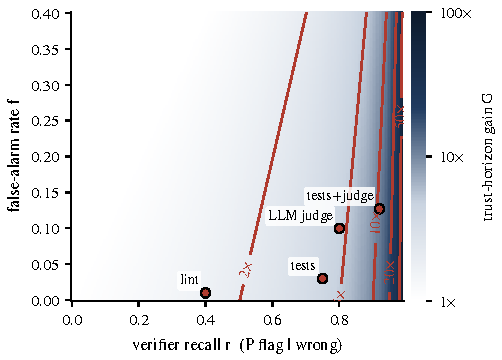
\includegraphics[width=\columnwidth]{figs_ieee/fig_gain.pdf}
\caption{Trust-horizon gain $G$ for a sensor with recall $r$ and false-alarm rate $f$ (unlimited retries, $\varepsilon=0.01$). Markers denote the illustrative sensor configurations of Table~\ref{tab:sensors}; their parameters are assumptions.}
\label{fig:gain}
\end{figure}

\subsection{Error Laundering Under Retries}\label{sec:laundering}
Proposition~\ref{prop:verifier} assumes independent retries. In practice, an agent that misinterprets a requirement often does so identically on every attempt. A step is called \emph{stuck} if every attempt produces the same incorrect output.

\begin{proposition}[Error laundering]\label{prop:laundering}
Let a step be stuck with probability $\varphi$, and let sensor verdicts be independent across attempts, as for a sampled language-model judge or a nondeterministic test. Then
\begin{equation}\label{eq:laundering}
P(\text{silent}\mid\text{stuck})=1-r^m\ \xrightarrow{\,m\to\infty\,}\ 1.
\end{equation}
Let a success have value 1, an escalation value 0, and a silent error value $-w$. The marginal value of allowing a $j$th attempt is $(1-\varphi)(a-wb)\,c^{\,j-1}-w\,\varphi\,(1-r)\,r^{\,j-1}$. If $a>wb$ and $c<r$, as in any useful regime, it is negative for all $j>m^*$, where
\begin{equation}\label{eq:mstar}
m^*=1+\frac{\ln\!\big[(1-\varphi)(a-wb)\,/\,(w\,\varphi\,(1-r))\big]}{\ln(r/c)}.
\end{equation}
\end{proposition}

For a moderately difficult step ($\varepsilon=0.05$, $r=0.9$, $f=0.05$), a 2\% probability of being stuck, and a silent error that costs ten times the value of a success ($w=10$), $m^*\approx2.6$. Because $w$ enters (\ref{eq:mstar}) through a logarithm, the optimal retry budget changes only slowly with the cost of a silent error. Fig.~\ref{fig:laundering} shows that on ordinary steps retries saturate after two or three attempts, whereas on stuck steps the probability of accepting an incorrect output increases steadily with $m$.

\begin{remark}
Equation (\ref{eq:laundering}) requires independent verdicts. A deterministic check, such as a type checker or a fixed unit test, either detects a stuck error on every attempt or on none, so retries cannot launder errors past it. This gives a quantitative reason to prefer computational sensors wherever a deterministic check exists, consistent with practitioner guidance~\cite{bockeler2026b}.
\end{remark}

\begin{figure*}[!t]
\centering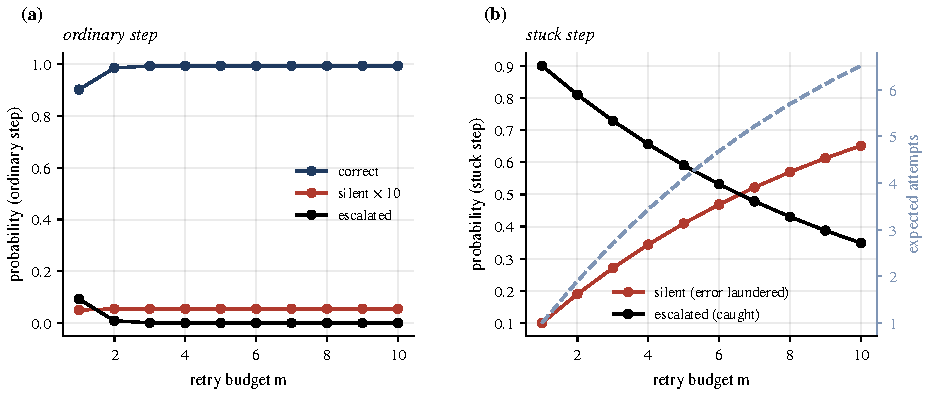
\includegraphics[width=\textwidth]{figs_ieee/fig_laundering.pdf}
\caption{Retry budgets. (a) Ordinary step ($\varepsilon=0.05$, $r=0.9$, $f=0.05$): success saturates by $m=3$. (b) Stuck step with a stochastic sensor: each retry increases the probability $1-r^m$ that an incorrect output is accepted, and the expected number of attempts (dashed, right axis).}
\label{fig:laundering}
\end{figure*}

\subsection{Context Degradation and a Square-Root Law for Resets}\label{sec:rot}
Context degradation is modeled as a linear increase in per-attempt error with steps since the most recent reset, $\varepsilon(s)=\varepsilon_0(1+\gamma s)$, so the error doubles after $1/\gamma$ steps. Without resets, $-\ln R(n)\approx\varepsilon_0 n+\tfrac12\varepsilon_0\gamma n^2$: reliability decays as a Gaussian rather than an exponential function of $n$, and the hazard increases with $n$. Resets bound this growth but risk losing state.

\begin{proposition}[Square-root law]\label{prop:sqrt}
With resets every $L$ steps and handoff loss $\rho$ per reset, the per-step hazard is, to first order,
\begin{equation}\label{eq:resethazard}
h(L)=\varepsilon_0+\tfrac12\varepsilon_0\gamma(L-1)+\frac{\rho}{L},
\end{equation}
which is minimized at
\begin{equation}\label{eq:lstar}
L^*=\sqrt{\frac{2\rho}{\varepsilon_0\gamma}},\qquad h(L^*)\approx\varepsilon_0+\sqrt{2\varepsilon_0\gamma\rho}.
\end{equation}
\end{proposition}

Equation (\ref{eq:lstar}) has the form of Young's optimal checkpoint interval, $\tau^*=\sqrt{2\delta M}$, for checkpoint cost $\delta$ and mean time between failures $M$~\cite{young1974,daly2006}. Here the cost of a reset is the probability of losing state in the handoff, and the failure rate is the rate at which degradation accumulates. The law agrees with simulation (Fig.~\ref{fig:sqrt}). Two practical consequences follow. First, the hazard is U-shaped in $L$, so resetting too often is as harmful as resetting too rarely. Second, because a sensor rescales $\varepsilon_0$ to $\et$, adding one shifts the optimum: $L^*_{\mathrm{verified}}/L^*_{\mathrm{bare}}=\sqrt{G}$. With $G=9.5$ the optimal interval increases from 20 to 62 steps in the reference setting, so a compaction policy tuned before a sensor is introduced is miscalibrated afterwards.

\begin{figure}[!t]
\centering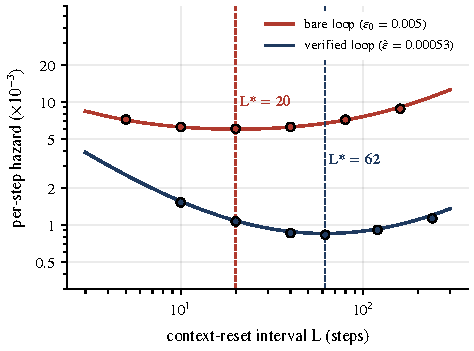
\includegraphics[width=\columnwidth]{figs_ieee/fig_sqrt.pdf}
\caption{Per-step hazard versus reset interval for a bare loop ($\varepsilon_0=0.005$) and a verified loop ($r=0.9$, $f=0.05$), with $\gamma=0.01$ and $\rho=0.01$. Lines: (\ref{eq:resethazard}); markers: simulation (20\,000 tasks per point); dashed lines: $L^*$ from (\ref{eq:lstar}).}
\label{fig:sqrt}
\end{figure}

\subsection{Checkpoints and Rerun Cost}\label{sec:checkpoints}
Agent errors typically remain silent until checked. If a task is checked only at completion, at cost $v$, and rerun on failure, the expected work is $(n+v)/p^n$, which is exponential in $n$.

\begin{proposition}[Checkpointing]\label{prop:ckpt}
With per-step success probability $p=e^{-h}$, a perfect segment check of cost $v$ every $L$ steps, and rollback on failure, the expected work is
\begin{equation}\label{eq:ckpt}
W(n)=\frac{n}{L}\cdot\frac{L+v}{p^{L}},\qquad L_c^*=\frac{-v+\sqrt{v^2+4v/h}}{2}\approx\sqrt{v/h},
\end{equation}
which is linear in $n$ and again has a square-root optimum.
\end{proposition}

For $p=0.99$ and $v=5$, $L_c^*\approx20$, and a 1000-step task requires about 1530 step-equivalents rather than $2.3\times10^7$ (Fig.~\ref{fig:checkpoint}). Checkpoints alone do not, however, confer trust. If the segment check has recall $r_s<1$, a silent error passes it with probability $\sigma=(1-p^L)(1-r_s)/[p^L+(1-p^L)(1-r_s)]$ per accepted segment, and end-to-end reliability remains $(1-\sigma)^{n/L}$, geometric in $n$. Checkpoints reduce cost; sensors increase trust. The long-running harness described in~\cite{anthropic2025long}, which commits tested progress to version control and records it in a progress file for subsequent sessions, combines both.

\begin{figure}[!t]
\centering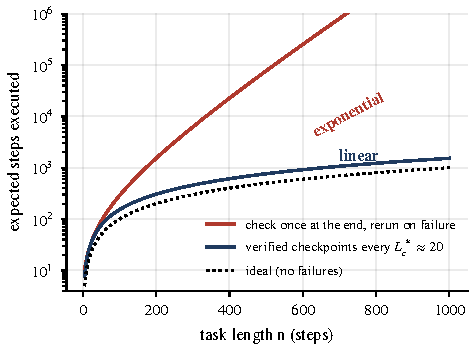
\includegraphics[width=\columnwidth]{figs_ieee/fig_checkpoint.pdf}
\caption{Expected work to complete a task ($p=0.99$, check cost $v=5$). A single terminal check with full reruns grows exponentially; verified checkpoints at $L_c^*\approx20$ grow linearly, at about $1.5\times$ the ideal.}
\label{fig:checkpoint}
\end{figure}

\subsection{The Trust Horizon Equation}\label{sec:the}
Combining Propositions~\ref{prop:verifier} and~\ref{prop:sqrt}, with $\varepsilon_0$ replaced by the silent-error rate $\et$ and the reset interval re-optimized, and adding the detected-failure floor due to escalation, gives the central approximation:
\begin{equation}\label{eq:the}
n^*_{\alpha}\approx\frac{\ln(1/\alpha)}{\et+\sqrt{2\,\et\,\gamma\,\rho}+f^{\,m}},\qquad \et=\varepsilon_0\,\frac{1-r}{1-f},
\end{equation}
with optimal reset interval $L^*=\sqrt{2\rho/(\et\gamma)}$. The three denominator terms are the errors that pass the sensor, the combined cost of context degradation and lossy handoffs, and the false-alarm floor. The expression holds in the small-error regime and uses $c^m\approx f^m$, which requires $\varepsilon\ll f$. Handoff loss is not discounted by recall (A5), because a step-level sensor evaluates whether an action was correct given its context, not whether the context retains the information required. Discounting $\rho$ by $(1-r)$ would overstate the horizon: at $r=0.99$ in the reference setting it predicts $n_{0.8}\approx3550$, against 1533 in simulation and 1438 from (\ref{eq:the}).

\begin{corollary}[Two regimes]\label{cor:regimes}
When $\et\gg2\gamma\rho$ the loop is verification-limited: $n^*_\alpha\propto1/\et\propto(1-r)^{-1}$, and halving the sensor's miss rate $1-r$ doubles the horizon. When $\et\ll2\gamma\rho$ it is memory-limited: $n^*_\alpha\approx\ln(1/\alpha)/\sqrt{2\et\gamma\rho}\propto(1-r)^{-1/2}\rho^{-1/2}$, so a tenfold reduction in the miss rate yields only about a $3.2\times$ longer horizon, and a proportional reduction in handoff loss yields the same return. The regimes meet at $\et=2\gamma\rho$.
\end{corollary}

In the reference setting ($\varepsilon_0=0.005$, $\gamma=\rho=0.01$), the transition occurs at $r\approx0.96$ (Fig.~\ref{fig:returns}). Beyond it, sensor recall and handoff fidelity enter the horizon almost symmetrically, so handoff fidelity, which no step-level sensor addresses, is as important a lever as further gains in recall. This is consistent with current practice in long-running harnesses, which invest in structured progress files, commits after each tested step, and initialization into a known environment state~\cite{anthropic2025long,lopopolo2026}.

\begin{figure}[!t]
\centering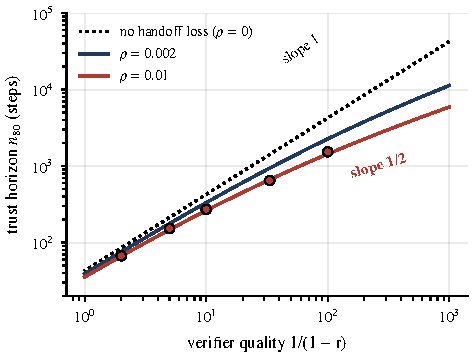
\includegraphics[width=\columnwidth]{figs_ieee/fig_returns.pdf}
\caption{Trust horizon versus sensor quality $1/(1-r)$ at the re-optimized reset interval. Without handoff loss (dotted) the slope is 1; with $\rho>0$ it approaches $1/2$. Markers: simulation at $\rho=0.01$.}
\label{fig:returns}
\end{figure}

% =====================================================================================
\section{Simulation Study}\label{sec:sim}

\subsection{Simulator}
Definition~\ref{def:model} was implemented as a vectorized Monte Carlo simulator in Python and NumPy (Appendix~\ref{app:sim}). Each run simulates between 8000 and 50\,000 independent tasks step by step and records the step and type (silent or escalated) of the first failure, so a single run yields the full survival curve $R(n)$. Cost is measured in generation-attempt units: one per attempt, plus $v$ per sensor invocation and a fixed charge per reset. Table~\ref{tab:params} lists the reference parameters, which were chosen to make each effect visible; they were not estimated from any deployed agent. Approximately $10^6$ synthetic tasks were simulated in total. Because the simulator implements the same model as the closed forms, agreement between the two checks the derivations and the accuracy of the approximations; it is not evidence that the model describes real agents. The code, outputs, and a script that checks every simulated number in this paper are available at \url{https://github.com/big-oh/trust-horizon}.

\begin{table}[!t]
\centering
\caption{Reference Simulation Parameters}
\label{tab:params}
\footnotesize
\begin{tabularx}{\columnwidth}{@{}llX@{}}
\toprule
Symbol & Value & Meaning\\
\midrule
$\varepsilon_0$ & 0.005 & per-attempt error immediately after a reset\\
$\gamma$ & 0.01 & error doubles after 100 steps without reset\\
$\rho$ & 0.01 & handoff loss per reset (0.002 in the improved-handoff condition)\\
$r,f$ & 0.9, 0.05 & reference sensor recall and false-alarm rate\\
$m$ & 3 & retry budget per step\\
$v$ & 0.3 & sensor cost per attempt\\
-- & 2 & cost of one context reset\\
Tasks & 8000--50\,000 & per condition; 95\% bootstrap intervals on $n_{0.8}$ within $\pm$2 steps for $n_{0.8}<50$ and $\pm$5\% otherwise\\
\bottomrule
\end{tabularx}
\end{table}

\subsection{Validation of Closed Forms}
Table~\ref{tab:validation} compares each closed-form prediction with simulation. The largest discrepancy, 7\%, occurs at the highest recall, where the first-order expansion in Proposition~\ref{prop:sqrt} is least accurate.

\begin{table*}[!t]
\centering
\caption{Closed-Form Predictions Versus Monte Carlo Simulation}
\label{tab:validation}
\small
\setlength{\tabcolsep}{4.5pt}
\begin{tabular}{@{}lllcc@{}}
\toprule
Result & Quantity & Setting & Predicted & Simulated\\
\midrule
Prop.~\ref{prop:invariance} & $R(100)$ & $\varepsilon=0.01$ & 0.366 & 0.363\\
Prop.~\ref{prop:frailty} & $T_{0.8}/T_{0.5}$ & Gamma frailty, $\nu=1$ & 0.250 & 0.240\\
Prop.~\ref{prop:verifier} & $n_{0.8}$ & $(r,f)=(0.5,0.02)$, $m=50$ & 43.4 & 43\\
 & & $(r,f)=(0.8,0.05)$, $m=50$ & 105.0 & 107\\
 & & $(r,f)=(0.9,0.05)$, $m=50$ & 210.0 & 209\\
 & & $(r,f)=(0.97,0.10)$, $m=50$ & 662.8 & 653\\
Prop.~\ref{prop:laundering} & $P(\mathrm{silent}\mid\mathrm{stuck})$ & $r=0.9$, $m=6$ & 0.469 & 0.471\\
Prop.~\ref{prop:sqrt} & $h(L)\times10^3$ & $L=5,10,20,40,80$ & 7.10, 6.23, 5.97, 6.23, 7.10 & 7.10, 6.24, 6.01, 6.22, 7.11\\
Eq.~(\ref{eq:the}) & $n_{0.8}$ & $r=0.5,0.9,0.99$; $\rho=0.01$; $L=L^*$; $m=200$ & 66, 262, 1438 & 67, 271, 1533\\
\bottomrule
\end{tabular}
\end{table*}

\subsection{Ablation of Harness Controls}\label{sec:ablation}
Controls were added one at a time to a bare loop in the reference setting (Fig.~\ref{fig:ablation}). Four findings emerge; they describe this setting and are not general claims.

\emph{Resets alone do not improve trust.} They extend the 50\% horizon from 95 to 118 steps but leave the 80\% horizon essentially unchanged (38 to 39), because degradation becomes significant only after about $1/\gamma=100$ steps, by which point a bare loop has usually failed. Context management helps only once other controls make long runs survivable.

\emph{The sensor is the largest single lever.} The reference sensor increases the trust horizon by a factor of 4.8 (38 to 184). This is below the unconstrained gain of 9.5 because degradation is active over the longer horizon and escalations add a failure floor.

\emph{Controls must be tuned jointly.} Adding resets at the interval that is optimal for the bare loop ($L=20$) slightly reduces the trust horizon (184 to 180). Re-tuning to $L^*=62$, as Proposition~\ref{prop:sqrt} predicts, increases it to 224.

\emph{Handoff fidelity adds a further gain.} A fivefold reduction in handoff loss increases the horizon to 267, more than any change in reset interval. The gain is moderate because at $r=0.9$ the loop is still verification-limited ($r<0.96$). The complete harness extends the trust horizon by a factor of 7.0. Every simulated horizon lies within 7\% of the corresponding closed-form prediction from Section~\ref{sec:model}.

\begin{figure*}[!t]
\centering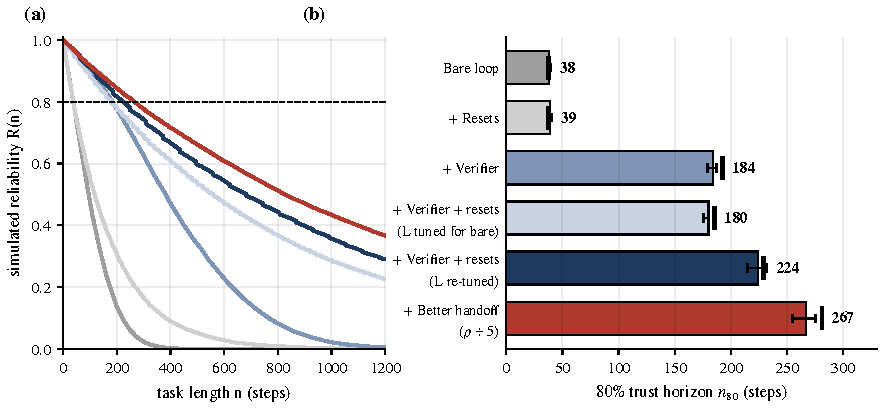
\includegraphics[width=\textwidth]{figs_ieee/fig_ablation.pdf}
\caption{Ablation of harness controls. (a) Simulated survival curves, shaded as in (b). (b) 80\% trust horizon with 95\% bootstrap intervals (20\,000 tasks per condition); black ticks denote the closed-form predictions of Section~\ref{sec:model} (Eq.~(\ref{eq:the}) for the conditions with a sensor and resets).}
\label{fig:ablation}
\end{figure*}

\subsection{Cost--Reliability Frontier}\label{sec:pareto}
A 150-step task was simulated under five illustrative sensor configurations (Table~\ref{tab:sensors}), four retry budgets ($m=1,2,3,5$), and resets enabled ($L=20$) or disabled, for 34 configurations in total (Fig.~\ref{fig:pareto}). The sensor parameters are assumptions chosen to span cheap low-recall checks to expensive high-recall ones.

\begin{table}[!t]
\centering
\caption{Illustrative Sensor Configurations (Assumed)}
\label{tab:sensors}
\footnotesize
\begin{tabular}{@{}lccc@{}}
\toprule
Sensor & Recall $r$ & False alarm $f$ & Cost $v$\\
\midrule
None & -- & -- & 0\\
Linter & 0.40 & 0.01 & 0.05\\
Unit tests & 0.75 & 0.03 & 0.25\\
LLM judge & 0.80 & 0.10 & 0.60\\
Tests + judge & 0.92 & 0.127 & 0.85\\
\bottomrule
\end{tabular}
\end{table}

With $m=1$, success falls to 0--10\% for every sensor, because each false alarm over 150 steps ends the task; a strong judge with $m=1$ achieves 0\%, compared with 26.5\% for no sensor. Verification reduces cost per successful task: unit tests with $m=3$ raise per-step cost by 30\% but reduce cost per success by about 30\%, because fewer runs are wasted. Inexpensive deterministic sensors dominate the lower part of the frontier: tests reach 71--75\% success at $1.6\times$ the ideal cost per success, whereas the judge alone costs more for comparable success. Combining tests and judge gives the highest success (88.5\%) and reduces the share of tasks ending in silent failure from 73.5\% to 10.8\%, at about $2.3\times$ ideal cost.

The numerical values depend on the assumed sensor parameters. Three qualitative features follow from the closed forms rather than from those values: false alarms require a retry budget (the $f^m$ floor), recall determines trust (the gain $G$), and sensor cost must be judged per successful task rather than per step.

\begin{figure*}[!t]
\centering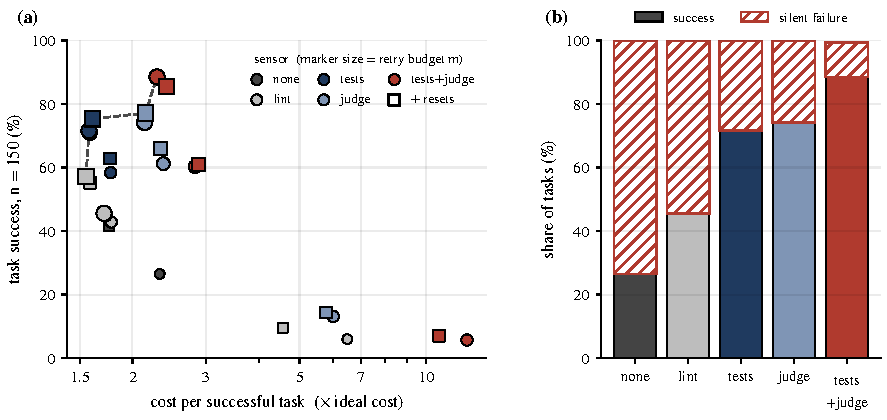
\includegraphics[width=\textwidth]{figs_ieee/fig_pareto.pdf}
\caption{Cost--reliability frontier for a 150-step task. (a) Success versus expected cost per successful task; dashed line: Pareto frontier. Configurations below 2\% success, which include every sensor other than the linter with $m=1$, are omitted. (b) Outcomes for the best configuration of each sensor without resets: success (solid) and silent failure (hatched). Sensor parameters (Table~\ref{tab:sensors}) are illustrative assumptions.}
\label{fig:pareto}
\end{figure*}

% =====================================================================================
\section{Implications for Harness Design}\label{sec:implications}
If the model's functional forms hold for real agents, which is the subject of Section~\ref{sec:program}, they imply seven design principles.
\begin{enumerate}
  \item Measure reliability per step as well as per task, and classify each failure as silent or detected; trust is determined by the silent fraction.
  \item Report $n_{0.8}$ and pass$^k$ alongside pass@1 and $n_{0.5}$; capability metrics cannot reveal the run-versus-trust gap, and pass$^k$ is the only routine metric sensitive to task heterogeneity.
  \item Prioritize sensor recall, and prefer computational sensors wherever a deterministic check exists; the gain is approximately $(1-f)/(1-r)$, and deterministic checks do not launder errors.
  \item Pair every sensor with a bounded retry budget followed by escalation, large enough that the false-alarm floor $f^m$ is small relative to $\et$ (three attempts for $f=0.03$ and five for $f\approx0.13$ in Section~\ref{sec:pareto}); under error laundering the optimal budget depends only logarithmically on the cost of a silent error.
  \item Re-tune compaction or reset intervals whenever the sensor changes; the optimal interval scales as $1/\sqrt{\et}$.
  \item In the memory-limited regime, treat handoff fidelity as a first-order lever: the horizon scales as $(\et\rho)^{-1/2}$, so reducing $\rho$ pays as much as the same proportional reduction in the miss rate.
  \item Checkpoint verified progress to turn exponential rerun cost into linear cost, recognizing that checkpoints do not substitute for sensors.
\end{enumerate}
For organizations practicing site reliability engineering, these principles correspond to an error budget per task, reliability targets expressed in nines per step, and failure modes that are designed rather than discovered~\cite{beyer2016}.

% =====================================================================================
\section{Proposed Empirical Validation}\label{sec:program}
The model is useful only if its parameters can be measured on real agents and its predictions survive testing. This section specifies the hypotheses, the observations that would refute them, and a measurement protocol.

\subsection{Hypotheses}
Table~\ref{tab:hyp} lists six hypotheses with their refutation criteria.

\begin{table*}[!t]
\centering
\caption{Falsifiable Hypotheses and Refutation Criteria}
\label{tab:hyp}
\small
\begin{tabularx}{\textwidth}{@{}p{0.6cm}XX@{}}
\toprule
 & Hypothesis & Refuted if\\
\midrule
H1 & Within a task instance, per-step hazard is approximately constant over short horizons; departures are explained by degradation (increasing) and heterogeneity (apparent decrease). & Per-task survival curves from repeated trials exhibit a declining hazard comparable to the population curve.\\
H2 & The declining population hazard in agent time-horizon data arises mainly from selection due to task heterogeneity rather than within-task learning. & A frailty model fits repeated-trial data significantly worse than a within-task learning model (likelihood-ratio test, $p<0.01$).\\
H3 & The measured gain in $n_{0.8}$ from a sensor equals $(1-f)/(1-r)$, with $r$ and $f$ estimated from labeled step outputs. & Measured gain deviates from prediction by more than 25\% for two or more sensor types.\\
H4 & With a sampled language-model judge, the silent-error rate on difficult steps increases with the retry budget; with a deterministic sensor it does not. & No increase in silent errors from $m=2$ to $m=8$ with the stochastic judge.\\
H5 & The optimal compaction or reset interval scales as $1/\sqrt{\et}$: introducing a sensor with gain $G$ shifts it by approximately $\sqrt{G}$. & The optimum does not shift, or shifts by less than half the predicted factor.\\
H6 & The sensitivity of $n_{0.8}$ to handoff loss grows with sensor recall: the elasticity of $n_{0.8}$ with respect to $\rho$ moves from near 0 (verification-limited) toward $-1/2$ (memory-limited). & The measured elasticity does not increase in magnitude between a configuration below and one above the estimated transition recall, in two or more task families.\\
\bottomrule
\end{tabularx}
\end{table*}

\subsection{Protocol}
The protocol requires tasks whose intermediate states can be verified automatically, so that each step can be labeled correct or incorrect independently of the agent's own sensors (Fig.~\ref{fig:protocol}). Three task families are proposed: multi-stage data transformations with a verifiable table after each stage; sequential refactoring chains with a unit test per step; and stateful tool-use tasks, in the style of $\tau$-bench, in which the database state after each action can be checked. Chaining short verified units makes task length a controlled variable, which existing benchmarks do not provide.

The design comprises two or three models, including at least one open-weights model; six task lengths from 4 to 128 steps; at least 30 task instances per length; at least eight repetitions per instance, for pass$^k$ and the frailty test; and a factorial harness grid over sensor type, retry budget, and reset interval. Parameters are estimated on half of the task lengths, and predictions are evaluated on the rest. Specifically, $\varepsilon_0$ is estimated from step labels immediately after resets; $\gamma$ from the slope of step error against context age; $r$ and $f$ from sensor verdicts against ground-truth labels; $\rho$ from failures on the first step after a reset that are attributable to missing state; and $\kappa$ from the Beta fit to repeated trials (Proposition~\ref{prop:passk}).

\begin{figure*}[!t]
\centering
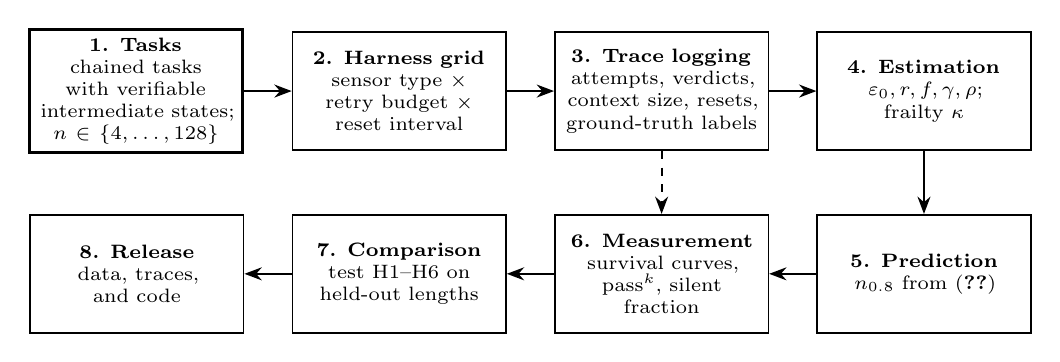
\begin{tikzpicture}[font=\scriptsize,
  bx/.style={draw=black,line width=0.6pt,align=center,text width=25mm,minimum height=15mm,fill=white,inner sep=3pt},
  ar/.style={-{Stealth[length=2.2mm]},line width=0.7pt}, node distance=6mm]
  \node[bx,line width=1.2pt] (t) {\textbf{1. Tasks}\\ chained tasks with verifiable intermediate states; $n\in\{4,\dots,128\}$};
  \node[bx,right=of t] (h) {\textbf{2. Harness grid}\\ sensor type $\times$ retry budget $\times$ reset interval};
  \node[bx,right=of h] (l) {\textbf{3. Trace logging}\\ attempts, verdicts, context size, resets, ground-truth labels};
  \node[bx,right=of l] (e) {\textbf{4. Estimation}\\ $\varepsilon_0,r,f,\gamma,\rho$; frailty $\kappa$};
  \node[bx,below=8mm of e] (p) {\textbf{5. Prediction}\\ $n_{0.8}$ from (\ref{eq:the})};
  \node[bx,left=of p] (m) {\textbf{6. Measurement}\\ survival curves, pass$^k$, silent fraction};
  \node[bx,left=of m] (c) {\textbf{7. Comparison}\\ test H1--H6 on held-out lengths};
  \node[bx,left=of c] (o) {\textbf{8. Release}\\ data, traces, and code};
  \draw[ar] (t)--(h); \draw[ar] (h)--(l); \draw[ar] (l)--(e); \draw[ar] (e)--(p); \draw[ar] (p)--(m); \draw[ar] (m)--(c); \draw[ar] (c)--(o);
  \draw[ar,dashed] (l.south) -- ++(0,-4mm) -| (m.north);
\end{tikzpicture}
\caption{Measurement protocol. Parameters estimated on one set of task lengths are used to predict survival on held-out lengths, providing an out-of-sample test of the model.}
\label{fig:protocol}
\end{figure*}

% =====================================================================================
\section{Limitations and Threats to Validity}\label{sec:limits}
\emph{No real-agent measurements:} All results are analytical or simulated, and the parameter values are illustrative. Agreement between closed forms and simulation confirms the derivations under Definition~\ref{def:model}; it does not show that real agents follow the model. The value of the model depends on confirmation of its functional forms under the protocol of Section~\ref{sec:program}.

\emph{Definition of a step:} METR measures task length in human minutes, whereas this model uses agent steps. The relation between the two is task-dependent and probably nonlinear; connections drawn to METR's data concern the shape of the curves, not their units.

\emph{Independence and recovery:} Errors may be correlated across steps (an incorrect plan affects many later steps), and sensors may share the generator's blind spots, reducing effective recall exactly where it matters. Propositions~\ref{prop:frailty} and~\ref{prop:laundering} relax independence in two specific forms; other dependence structures are not treated. Conversely, assumption (A1) ignores late recovery from silent errors, which would lengthen horizons.

\emph{Linear degradation:} The form $\varepsilon_0(1+\gamma s)$ is the simplest assumption consistent with the evidence~\cite{hong2025}; degradation may be nonlinear, task-dependent, or partly offset by adaptation to the environment.

\emph{Tension with declining hazards:} The model predicts increasing per-task hazard from degradation, whereas population data show declining hazard. Heterogeneity can mask the former, and deployed harnesses already manage context, but the tension is unresolved; it is the subject of H1 and H2.

\emph{Cost model:} Costs are counted in attempt units with fixed sensor and reset charges; token costs that grow with context length and the cost of human review of escalations are not modeled.

\emph{Literature figures:} Harness-variance comparisons are observational; the $\tau$-bench values fitted here come from the repository leaderboard on the original task set, which was later revised; and several 2026 sources are preprints or practitioner reports that have not been peer reviewed. These figures motivate the model but do not test it.

\emph{Sensor parameters:} The recall, false-alarm, and cost values in Section~\ref{sec:pareto} are assumptions; their measurement is part of the proposed protocol.

% =====================================================================================
\section{Open Questions}\label{sec:open}
Six questions remain open. \emph{Selection or learning:} is the declining hazard observed in agents a property of the agents or of the task distribution? \emph{Step calibration:} can agent steps be mapped to human-equivalent time so that per-step reliabilities translate into time horizons? \emph{Generator--judge correlation:} if a model and its judge share failure modes, effective recall on difficult steps may be far below measured recall. \emph{Handoff loss:} can $\rho$ be measured directly for compaction, summaries, progress files, and commits? \emph{Harness transfer:} does a harness's gain transfer across model families, or is part of the observed variance a model--harness interaction? \emph{Tail reliability:} current data cannot discriminate between survival models whose implied 99\% horizons differ by more than an order of magnitude; an experimental design that can do so is needed.

% =====================================================================================
\section{Conclusion}\label{sec:conclusion}
The gap between what agents can do and what they can be trusted to do is consistent with series reliability applied to a loop of fallible steps, compounded by heterogeneity across tasks and degradation of context. Better models raise all horizons proportionally but do not, alone, change the ratio between capability and trust. A reliability model with one parameter per harness component reproduces the observed ratio, shows that sensors multiply the trust horizon whereas checkpoints reduce the cost of failure, identifies the error-laundering risk of unbounded retries against stochastic sensors, and predicts that once verification is strong, handoff fidelity matters as much as sensor recall. These are predictions of a model, not measurements; each can be tested with the protocol described.

% =====================================================================================
\appendices
\section{Proofs}\label{app:proofs}
\emph{Proposition~\ref{prop:invariance}:} Independent steps give $R(n)=(1-\varepsilon)^n$. Setting $R(n)=\alpha$ gives $n_\alpha=\ln\alpha/\ln(1-\varepsilon)$, and the ratio of two such expressions eliminates $\ln(1-\varepsilon)$. The approximation uses $-\ln(1-\varepsilon)=\varepsilon+O(\varepsilon^2)$.\hfill$\blacksquare$

\emph{Proposition~\ref{prop:frailty}:} Conditional on $\lambda$, survival is $e^{-\lambda t}$. The Gamma Laplace transform gives $\E[e^{-\lambda t}]=(\omega/(\omega+t))^\nu$, and $h(t)=-\tfrac{d}{dt}\ln S=\nu/(\omega+t)$. Solving $S(T_\alpha)=\alpha$ gives $T_\alpha=\omega(\alpha^{-1/\nu}-1)$. At $\nu=1$, $T_{0.8}/T_{0.5}=0.25$ and $S(t)=1/(1+t/T_{0.5})$. As $\nu\to\infty$ with fixed median, $\alpha^{-1/\nu}-1\sim\ln(1/\alpha)/\nu$, so the ratio tends to $\ln1.25/\ln2$.\hfill$\blacksquare$

\emph{Proposition~\ref{prop:passk}:} By the Beta-function recurrence, $\E[\theta^k]=B(a+k,b)/B(a,b)=\prod_{j=0}^{k-1}(a+j)/(a+b+j)$, and $\passat{k}=1-\E[(1-\theta)^k]$ follows by symmetry. Since $\mathrm{Var}(\theta)=\mu(1-\mu)/(a+b+1)$ with $\mu=a/(a+b)$, $\kappa=1/(a+b+1)$. The fits in Table~\ref{tab:beta} solve $\mu=\mathrm{pass}^1$ and $\E[\theta^4]=\mathrm{pass}^4$ numerically.\hfill$\blacksquare$

\emph{Proposition~\ref{prop:verifier}:} Each attempt independently terminates in state $a$, $b$, or $c$ of (\ref{eq:abc}). The step ends with an acceptance at attempt $j\le m$ with probability $c^{j-1}(a+b)$; summing the geometric series yields (\ref{eq:step}), and the expected number of attempts is $\sum_{j=1}^{m}c^{j-1}$. Conditional on acceptance the error rate is $b/(a+b)$; expansion for small $\varepsilon$ gives (\ref{eq:gain}).\hfill$\blacksquare$

\emph{Proposition~\ref{prop:laundering}:} On a stuck step every attempt is incorrect and is flagged independently with probability $r$, so it is accepted before the budget is exhausted with probability $1-r^m$. Compare budgets $j$ and $j-1$: they differ only when attempt $j$ is reached, and without it the step escalates (value 0). On a non-stuck step, attempt $j$ is reached with probability $c^{j-1}$ and ends in a correct acceptance with probability $a$ (value 1) or a silent error with probability $b$ (value $-w$); on a stuck step it is reached with probability $r^{j-1}$ and ends in a silent error with probability $1-r$. This gives the stated marginal value, which is negative when $(c/r)^{j-1}<w\varphi(1-r)/[(1-\varphi)(a-wb)]$; taking logarithms with $c<r$ gives (\ref{eq:mstar}).\hfill$\blacksquare$

\emph{Proposition~\ref{prop:sqrt}:} Over one reset cycle, $-\ln R\approx\sum_{s=0}^{L-1}\varepsilon_0(1+\gamma s)+\rho=\varepsilon_0L+\tfrac12\varepsilon_0\gamma L(L-1)+\rho$, using $-\ln(1-x)\approx x$. Division by $L$ yields (\ref{eq:resethazard}). Setting $h'(L)=\tfrac12\varepsilon_0\gamma-\rho/L^2=0$ gives $L^*$, and $h(L^*)=\varepsilon_0(1-\gamma/2)+\sqrt{2\varepsilon_0\gamma\rho}$.\hfill$\blacksquare$

\emph{Proposition~\ref{prop:ckpt}:} Each segment attempt costs $L+v$ and succeeds with probability $p^L$; the number of attempts is geometric with mean $p^{-L}$, and there are $n/L$ segments. Minimizing $\ln(L+v)-\ln L+hL$ gives $h=1/L-1/(L+v)$, that is, $L^2+vL-v/h=0$.\hfill$\blacksquare$

\emph{Equation~(\ref{eq:the}):} With a sensor, the accepted-error rate at context age $s$ is $\et(1+\gamma s)$ to first order, so Proposition~\ref{prop:sqrt} applies with $\varepsilon_0$ replaced by $\et$. Handoff loss is a silent error not observed by the step sensor (A5) and is not scaled by $1-r$. Escalation contributes hazard $c^m\approx f^m$ per step. Summing the three hazards, which is valid when each is small, and applying (\ref{eq:horizon}) gives the result.\hfill$\blacksquare$

\section{Simulation Details}\label{app:sim}
The simulator implements Definition~\ref{def:model}. At each step it operates on all surviving tasks simultaneously: it applies a reset and handoff loss if due, computes $\varepsilon(s)$, draws up to $m$ attempts (stuck steps repeat their error), draws independent sensor verdicts, and records the first silent error or escalation. Context age advances once per step, not per attempt (A3). Task heterogeneity is introduced by drawing each task's $\varepsilon_0$ from a Gamma distribution with shape $\nu$ and mean $\varepsilon_0$. Bootstrap intervals resample tasks with 150 replicates. All experiments use fixed random seeds, and repeated runs produce identical output.

\section{Notation}\label{app:notation}
Table~\ref{tab:notation} summarizes the notation.

\begin{table}[!h]
\centering
\caption{Notation}
\label{tab:notation}
\footnotesize
\begin{tabularx}{\columnwidth}{@{}lX@{}}
\toprule
Symbol & Meaning\\
\midrule
$n$, $R(n)$ & task length in steps; probability of completing $n$ steps\\
$\nal$, $n^*_\alpha$ & trust horizon at reliability $\alpha$; its closed-form approximation\\
$\varepsilon_0$, $\et$ & per-attempt error after a reset; silent-error rate after verification\\
$r$, $f$ & sensor recall and false-alarm rate\\
$a$, $b$, $c$ & per-attempt probabilities of correct acceptance, silent error, rejection\\
$m$, $m^*$ & retry budget; its optimum under error laundering\\
$\varphi$, $w$ & probability that a step is stuck; cost of a silent error relative to a success\\
$\gamma$, $\rho$ & context-degradation rate; handoff loss per reset\\
$s$ & steps since the most recent reset (context age)\\
$L$, $L^*$ & reset interval and its optimum\\
$L_c^*$, $v$ & optimal checkpoint interval; sensor or check cost\\
$G$ & verification gain $\varepsilon/\et$\\
$h$ & hazard (per-step failure rate)\\
$\nu$, $\omega$ & shape and rate of the Gamma frailty distribution; $\nu$ also denotes a Weibull shape\\
$\theta$, $\kappa$ & per-task success probability; intra-task correlation\\
$k$ & number of trials in pass$^k$ and pass@$k$\\
\bottomrule
\end{tabularx}
\end{table}

\section*{Acknowledgment}
In accordance with IEEE policy on the use of artificial intelligence--generated content, the author discloses that Claude (Anthropic) was used to assist with the literature search, citation checking, mathematical derivations, simulation code, figure generation, and drafting and revision of all sections of this manuscript. The author reviewed the content and takes responsibility for it. No external funding was received.

\bibliographystyle{IEEEtran}
\bibliography{refs}

\end{document}
